\documentclass[12pt,a4paper]{article}
\usepackage{fontspec}
\usepackage{polyglossia}
\setdefaultlanguage{russian}
\setmainfont{STIX Two Text}[AutoFakeBold=1.5]
\setmonofont{Menlo}
\newfontfamily\cyrillicfonttt{Menlo}
\usepackage[a4paper,margin=2cm]{geometry}
\usepackage{graphicx,longtable,tabularx,array,booktabs}
\usepackage{float,caption,enumitem,pdflscape,xurl,listings,tikz}
\usepackage{hyperref,etoolbox}
\usetikzlibrary{positioning,arrows.meta}
\hypersetup{colorlinks=true,linkcolor=blue,urlcolor=blue}
\lstset{basicstyle=\ttfamily\footnotesize,breaklines=true,columns=fullflexible,frame=single,keepspaces=true,showstringspaces=false}
\setlength{\parindent}{1.25cm}
\setlength{\parskip}{0.25em}
\renewcommand{\arraystretch}{1.16}
\setlist{nosep,leftmargin=1.5em}
\AtBeginEnvironment{longtable}{\small}
\sloppy
\begin{document}
\begin{titlepage}
\centering
{\large Практическая работа\par}
\vspace{2.2cm}
{\LARGE\bfseries Отчёт по практической работе № 7\par}
\vspace{0.6cm}
{\Large Реализация безопасной аутентификации\par}
\vspace{1.8cm}
\begin{tabular}{p{4cm}p{11cm}}
Дисциплина: & Основы разработки защищённого программного обеспечения и компьютерных сетей\\
Вариант: & 19 — Система учёта транспортных средств организации\\
Исходная версия: & v0.6\\
Версия работы: & v0.7\\
Студент: & Мостовая Полина Андреевна\\
Группа: & ИУСбд-02-23
\end{tabular}
\vfill
{\large 2026\par}
\end{titlepage}
\tableofcontents
\clearpage

\section{Тема, цель и характеристика среды}
Тема работы — безопасная аутентификация в сквозном проекте учёта транспортных средств. Цель — реализовать регистрацию, парольную проверку, временную блокировку, серверные сеансы и одноразовое восстановление, затем проверить их автоматизированными сценариями. Работа продолжает v0.6, сохраняя её модули учёта обращений, файлового хранилища, RBAC и валидации.

Проверенная среда: macOS, Python 3.12.14 из виртуального окружения, pytest 9.0.2, SQLite из стандартной библиотеки, XeTeX (TeX Live 2026). Проект не имеет веб-интерфейса или сетевого API.

\section{Вариант 19 и границы реализации}
Индивидуальное задание — анализ риска блокировки чужой учётной записи. Нарушитель знает логин сотрудника, но не пароль; пять неверных попыток вызывают временный отказ владельцу при создании нового сеанса. Это злоупотребление средством защиты доступности. Brute Force проверяет много кандидатов для одной записи; Password Spraying — небольшое число типовых паролей для многих записей; вариант 19 не пытается угадать пароль.

AuthService подтверждает только серверный числовой \texttt{user\_id}. Он не назначает роль из пользовательского ввода и пока не подключён к сервисам автопарка. Будущая интеграция должна получать роль из серверного отображения подтверждённого id к RBAC. Это не веб-сервер и не MFA.

\section{Архитектура аутентификации}
SQLite предоставляет локальное хранилище, а ограниченные параметры запросов и транзакции используются стандартным интерфейсом Python. \cite{sqlite}
Вход начинается с недоверенных строк логина и пароля. После проверок SQLite возвращает соль, стоимость KDF и проверочное значение. PBKDF2 вычисляет кандидат, сравнение выполняется \texttt{hmac.compare\_digest}. Успех создаёт токен сеанса, но в БД записывается лишь SHA-256. При ошибке обновляется счётчик. Редактируемая схема: \texttt{docs/auth\_registration\_login.mmd}.

\begin{figure}[H]\centering
\resizebox{\textwidth}{!}{%
\begin{tikzpicture}[node distance=8mm and 9mm,box/.style={draw,rounded corners,align=center,text width=2.8cm,minimum height=12mm,font=\small},arrow/.style={-{Stealth},thick}]
\node[box] (client) {Клиент\\login/password};
\node[box,right=of client] (service) {AuthService\\валидация};
\node[box,right=of service] (kdf) {PBKDF2\\сравнение};
\node[box,above right=of kdf] (users) {SQLite users\\salt, rounds, hash};
\node[box,below right=of kdf] (sessions) {SQLite sessions\\token hash};
\node[box,right=of sessions] (result) {Сеансовый токен\\однократная выдача};
\draw[arrow] (client)--(service); \draw[arrow] (service)--(kdf); \draw[arrow] (kdf)--(users); \draw[arrow] (users)--(kdf); \draw[arrow] (kdf)--(sessions); \draw[arrow] (sessions)--(result);
\end{tikzpicture}}
\caption{Проверка пароля и создание серверного сеанса.}
\end{figure}

\section{Хранение паролей}
NFC-нормализация выполняется средствами стандартного модуля Unicode. \cite{unicode}
Принципы применения PBKDF2 и соли сверены с документацией Python и OWASP. \cite{hashlib,owasp-password}
Логин принимается только как \texttt{str}, нормализуется \texttt{casefold()}, затем проверяется шаблон \texttt{[a-z][a-z0-9\_]{2,31}}. Новый пароль нормализуется NFC; допустимая длина после нормализации — 15–128 символов, максимальный размер UTF-8 — 1024 байта. Пробелы не удаляются, регистр не меняется. Запрещающий список содержит лишь три учебных примера и не покрывает известные утечки.

Для каждого пароля используются 16 случайных байтов соли и PBKDF2-HMAC-SHA-256 с 600\,000 итераций и результатом 32 байта. В БД записывается и число итераций. SHA-256 слишком быстр для пароля с низкой энтропией; для случайного высокоэнтропийного токена быстрый SHA-256 используется как проверочное значение.

\section{Ограничение попыток и вариант 19}
Общий отказ при ошибке аутентификации рекомендован для уменьшения перечисления пользователей; счётчики попыток также требуют анализа риска блокировки. \cite{owasp-auth,nist}
После пяти последовательных ошибок блокировка действует 60 секунд. Правильный пароль до срока также не даёт новый сеанс. При точном равенстве времени границе блокировка окончена; успех сбрасывает счётчик. Неизвестный логин вызывает фиктивное вычисление KDF, которое уменьшает очевидное временное различие, но не исключает все тайминг-каналы.

Исследование использовало только временную локальную БД и искусственную запись с управляемыми часами. Проверены штатный вход владельца, пять неудач от другого участника, невозможность создать новый сеанс в течение блокировки, восстановление входа на границе 60 секунд и независимость другой учётной записи. Уже выданный сеанс этой блокировкой не отзывается. Ограничение затрудняет часть онлайн-подбора, но может использоваться для отказа в обслуживании конкретному владельцу.

Возможные будущие меры: ограничения источника и общей частоты, нарастающая задержка, сочетание нескольких сигналов, уведомление, challenge подозрительных попыток, контроль массовых обращений и безопасное восстановление доступности. Они предложены, но не реализованы. Фиксированные 60 секунд не являются универсальной защитой от распределённого подбора.

\section{Управление сеансами}
Случайная генерация токенов и серверное хранение их состояния соответствуют общим рекомендациям по сессиям. \cite{secrets,owasp-session}
Токен создаётся через \texttt{secrets.token\_urlsafe(32)}. Сервер хранит SHA-256, user id, время создания и последнюю активность. \texttt{resolve()} проверяет формат, активность учётной записи, абсолютный срок 3600 секунд и срок бездействия 900 секунд; при успехе обновляет \texttt{last\_seen}. \texttt{logout()} удаляет серверную запись. Удаление клиентской копии не отзывает скопированный токен. Схема: \texttt{docs/auth\_session.mmd}.

\section{Восстановление доступа}
Одноразовые коды, отзыв сеансов и отдельный последующий вход рассматриваются в материалах по восстановлению. \cite{owasp-recovery,nist}
При регистрации генерируется случайный recovery-код, который выдаётся вызывающей стороне однократно; БД хранит его SHA-256. Восстановление проверяет логин, код и новый пароль, заменяет соль, хеш пароля и хеш нового кода в транзакции и отзывает все сеансы. Новый сеанс автоматически не выдаётся; выполняется отдельный обычный вход. Старый код становится недействительным. Это учебная модель предварительно выданного кода, а не процесс подтверждения личности через канал связи. Схема: \texttt{docs/auth\_recovery.mmd}.

\section{Фрагменты исходного кода}
Реализация парольной KDF и recovery-проверочного значения:
\begin{lstlisting}[language=Python]
salt = secrets.token_bytes(16)
password_hash = hashlib.pbkdf2_hmac(
    "sha256", password_bytes, salt, self.rounds, dklen=32
)
recovery_hash = hashlib.sha256(recovery_code.encode("ascii")).digest()
\end{lstlisting}

Проверка пароля и серверная запись токена:
\begin{lstlisting}[language=Python]
candidate = self._derive(password_bytes, salt, rounds)
password_ok = hmac.compare_digest(candidate, stored)
token = secrets.token_urlsafe(32)
digest = self._token_hash(token)
db.execute("INSERT INTO sessions(token_hash,user_id,created,last_seen) VALUES(?,?,?,?)",
           (digest, row["id"], now, now))
\end{lstlisting}
Полный код находится в \texttt{app/auth.py}; фрагменты соответствуют версии v0.7.

\section{Результаты тестирования}
Тестовый экземпляр допускает 1000 итераций только для ускорения изолированных тестов; стандартное значение остаётся 600\,000. Полный локальный набор: 149 тестов и 9 subtests пройдены. Набор v0.7 содержит 29 тестов. Отдельный запуск демонстрации фактически выполнил регистрацию, вход и восстановление при 600\,000 итерациях.

\begin{longtable}{p{0.65cm}p{6.7cm}p{4cm}p{2.2cm}}
\toprule № & Сценарий & Ожидаемый результат & Факт \\
\midrule\endhead
1 & Правильный пароль & Вход разрешён & Пройдено \\
2 & Неверный пароль & Отказ & Пройдено \\
3 & Повторный логин & Отказ регистрации & Пройдено \\
4 & Равные пароли разных пользователей & Разные соли & Пройдено \\
5 & Проверка хранилища & Пароля в открытом виде нет & Пройдено \\
6 & Короткий пароль & Отклонён & Пройдено \\
7 & Добавочный пробел & Считается частью пароля & Пройдено \\
8 & Неизвестная запись & Отказ & Пройдено \\
9 & Пять ошибок & Временная блокировка & Пройдено \\
10 & Истечение блокировки & Вход на точной границе & Пройдено \\
11 & Выход & Токен отозван & Пройдено \\
12 & Срок бездействия & Сеанс недействителен & Пройдено \\
13 & Абсолютный срок & Сеанс недействителен & Пройдено \\
14 & Восстановление & Прежние сеансы отозваны & Пройдено \\
15 & Неверный recovery-код & Отказ без изменений & Пройдено \\
16 & Вариант 19: штатный вход & Успех до атаки & Пройдено \\
17 & Вариант 19: пять ошибок постороннего & Владелец временно заблокирован & Пройдено \\
18 & Вариант 19: истёкший срок & Вход восстановлен & Пройдено \\
19 & NFC и длина 15/128/129 & Нормализация и границы & Пройдено \\
20 & Размер UTF-8 и слабый пароль & Недопустимое отклонено & Пройдено \\
21 & Регистр логина и типы & Casefold и строгие типы & Пройдено \\
22 & Неверный токен и его хранение & Отказ; в БД только хеш & Пройдено \\
23 & Одноразовость recovery-кода & Повторный код отклонён & Пройдено \\
24 & Изоляция разных логинов & Другой вход доступен & Пройдено \\
25 & Сброс ошибок после успеха & Счётчик обнулён & Пройдено \\
26 & Обновление активности & Срок бездействия продлён & Пройдено \\
27 & Восстановление & Новый сеанс не создаётся & Пройдено \\
28 & Повреждённая соль & Безопасный отказ & Пройдено \\
29 & Уже действующий сеанс при блокировке новых входов & Не отзывается блокировкой & Пройдено \\
\bottomrule
\end{longtable}

\section{Ручные скриншоты}
Снимки получены из Terminal.app после запуска соответствующих режимов демонстрации. На них не видны пароли, резервные коды или действующие токены. Каждое изображение соответствует фактическому выводу локальной демонстрации и тестов.

\begin{figure}[H]\centering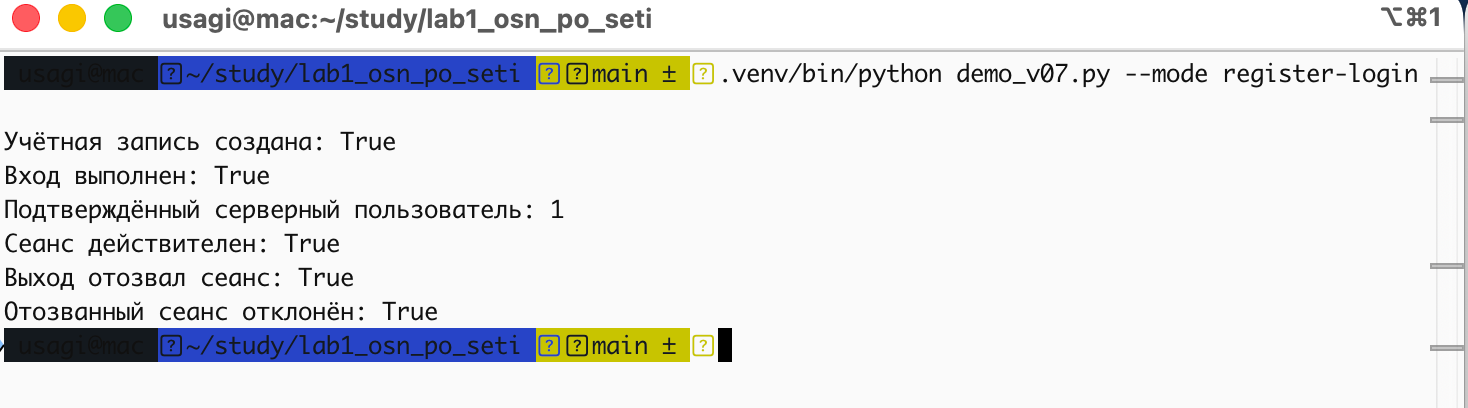
\includegraphics[width=\textwidth]{screenshots_manual/lab7_01_registration_login.png}\caption{Регистрация, вход, проверка серверной идентичности и отзыв сеанса.}\end{figure}
\begin{figure}[H]\centering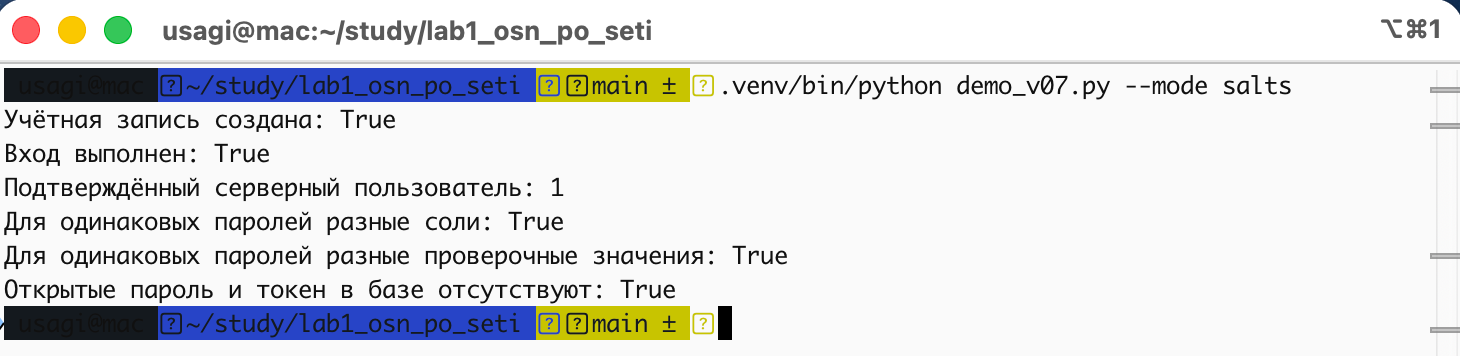
\includegraphics[width=\textwidth]{screenshots_manual/lab7_02_salts_hashes.png}\caption{Различие солей и парольных проверочных значений при одинаковом пароле.}\end{figure}
\begin{figure}[H]\centering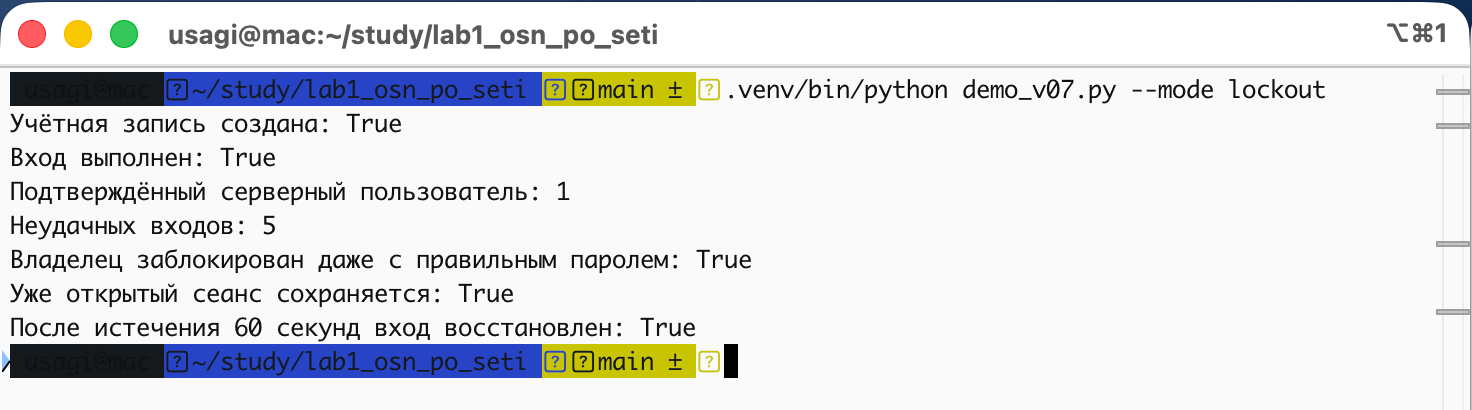
\includegraphics[width=\textwidth]{screenshots_manual/lab7_03_lockout.png}\caption{Пять неудачных попыток, отказ корректному паролю и истечение блокировки.}\end{figure}
\begin{figure}[H]\centering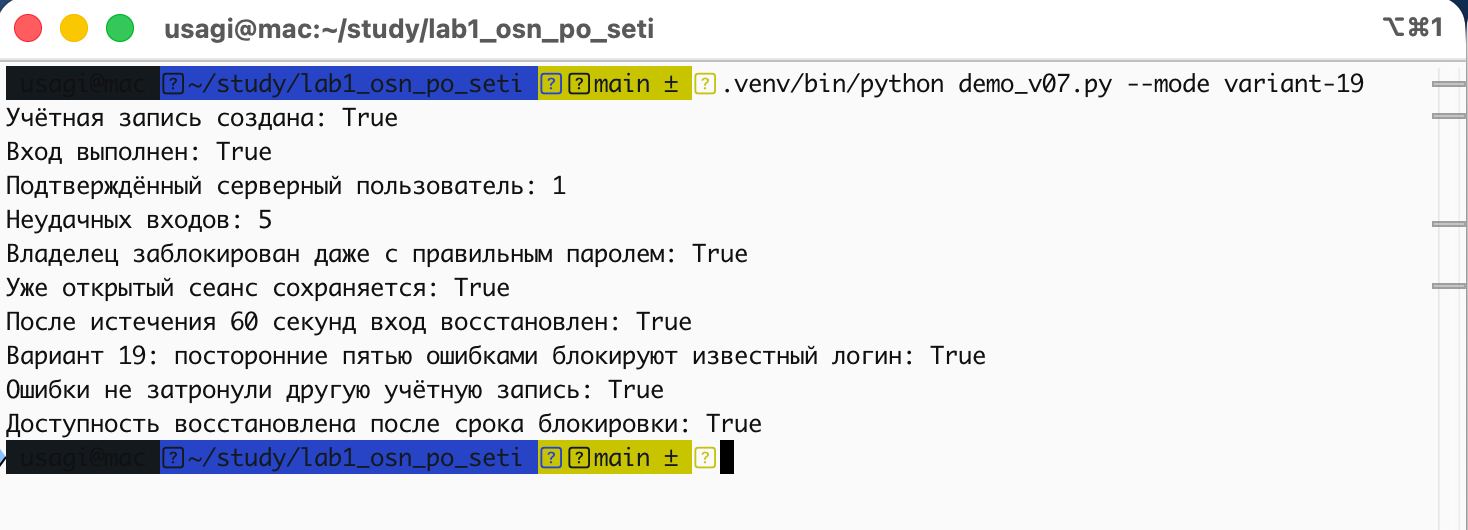
\includegraphics[width=\textwidth]{screenshots_manual/lab7_04_variant19.png}\caption{Вариант 19: блокировка чужого логина и восстановление доступности.}\end{figure}
\begin{figure}[H]\centering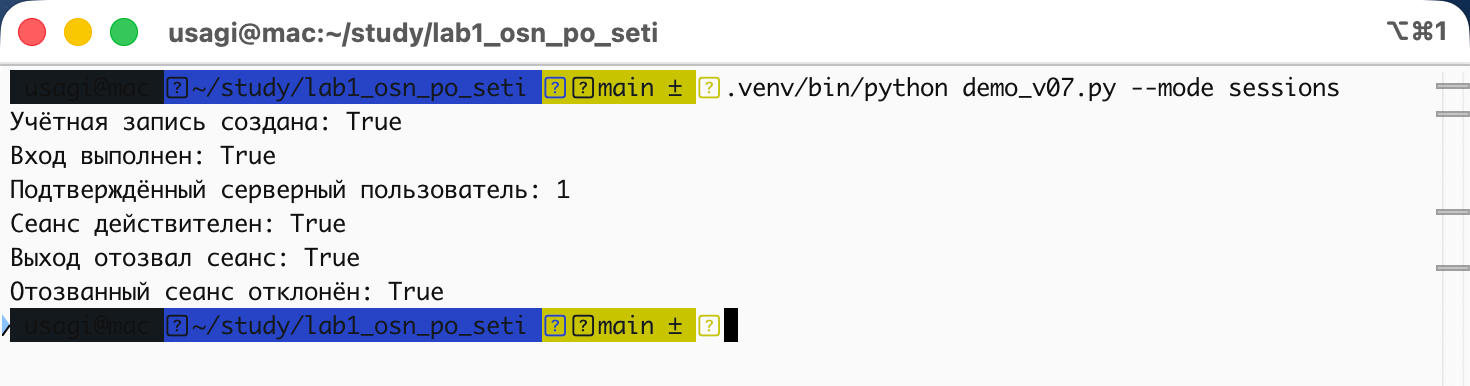
\includegraphics[width=\textwidth]{screenshots_manual/lab7_05_sessions.png}\caption{Проверка действующего сеанса и отказ после серверного отзыва.}\end{figure}
\begin{figure}[H]\centering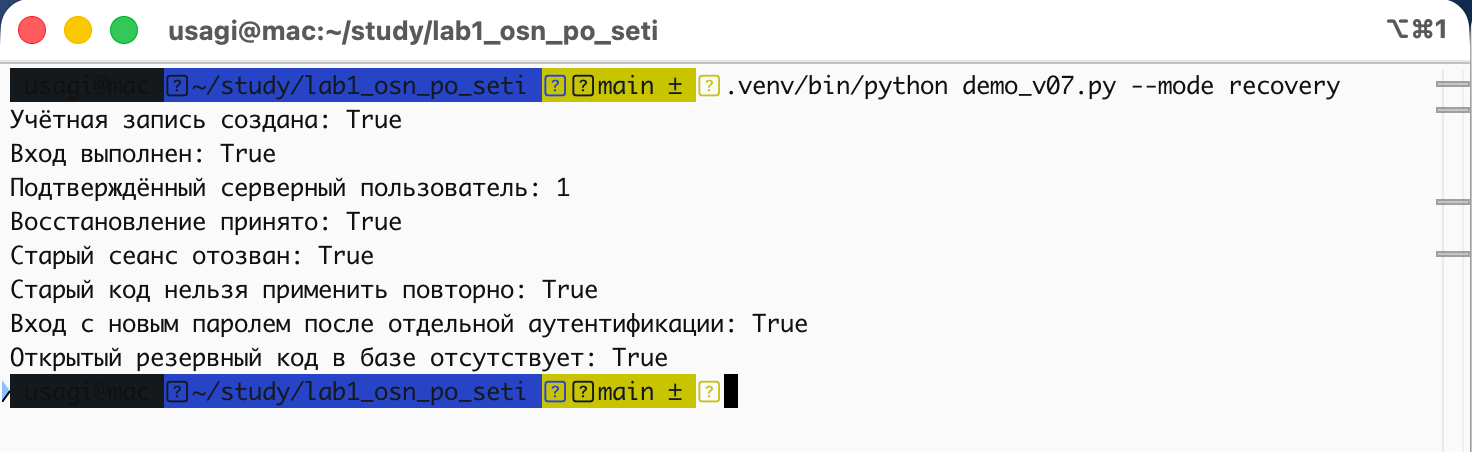
\includegraphics[width=\textwidth]{screenshots_manual/lab7_06_recovery.png}\caption{Одноразовое восстановление доступа и отзыв прежнего сеанса.}\end{figure}
\begin{figure}[H]\centering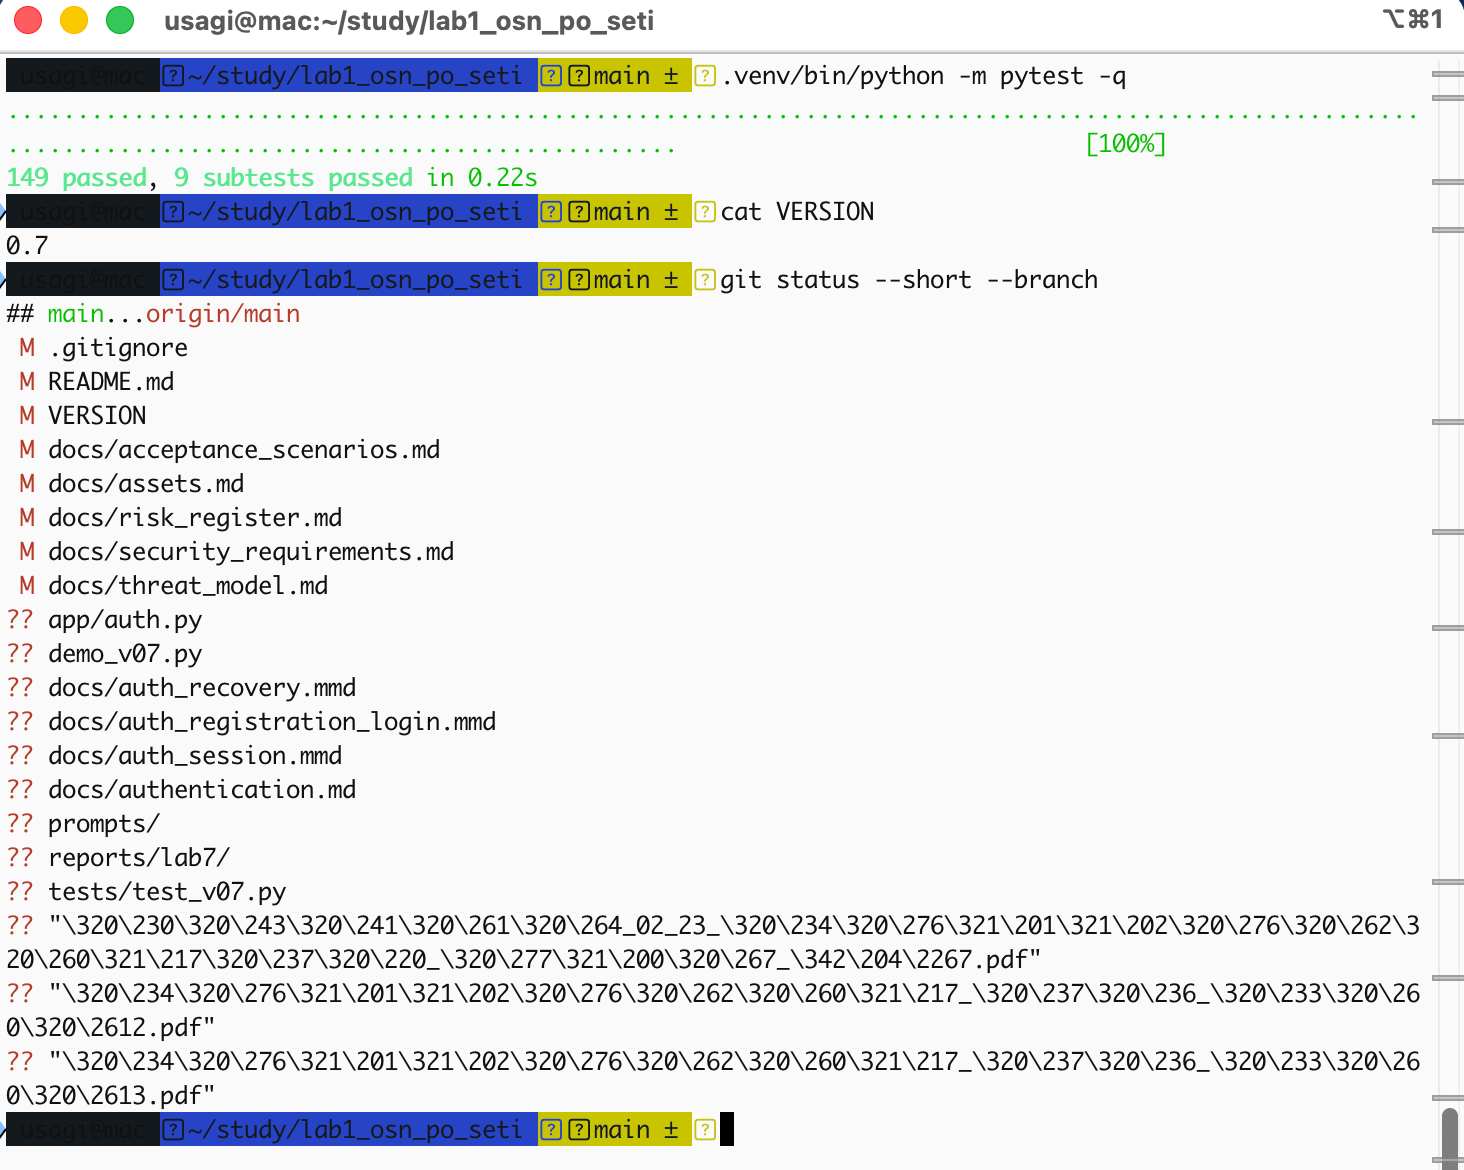
\includegraphics[width=0.84\textwidth]{screenshots_manual/lab7_07_tests_version.png}\caption{Фактические результаты регрессионных тестов, VERSION и состояние рабочей копии.}\end{figure}

\section{Остаточные риски}
Учебный список слабых паролей неполон; PBKDF2 не memory-hard; фиктивный KDF не устраняет все временные различия; блокировка создаёт отказ в доступности и не устраняет распределённый перебор. SQLite предназначена здесь для локального процесса и файла. Кража активного токена или recovery-кода остаётся значимой. Отсутствуют MFA, сетевое ограничение частоты, уведомления, подтверждённые каналы восстановления, назначение ролей и связь с бизнес-операциями автопарка.

\section{Вывод}
Создан локальный AuthService с индивидуальными солями, PBKDF2-HMAC-SHA-256, блокировкой после пяти ошибок, проверкой и отзывом сеансов, одноразовым восстановлением и отзывом прежних сеансов. Пройдены 149 регрессионных тестов и 9 subtests; стандартные 600\,000 итераций использованы в отдельной регистрации, входе и восстановлении. Вариант 19 исследован на искусственной локальной записи. Результаты ручных демонстраций подтверждены семью скриншотами, включёнными в отчёт.

\section{Ответы на контрольные вопросы}
\begin{enumerate}
\item Идентификация — указание рассматриваемой учётной записи.
\item Аутентификация проверяет доказательство контроля этой записи.
\item Открытый пароль после утечки сразу раскрывает секрет пользователя.
\item Соль — случайное значение, индивидуализирующее парольную проверку.
\item Разные соли скрывают совпадение проверочных значений равных паролей.
\item SHA-256 слишком быстр для перебора низкоэнтропийных паролей.
\item PBKDF2 — многократное преобразование пароля через HMAC для повышения стоимости проверки.
\item Argon2id использует память и вычисления, затрудняя параллельный массовый перебор.
\item \texttt{compare\_digest} снижает зависимость времени сравнения от общего префикса значений.
\item Пробел может быть частью секрета; его удаление меняет ввод.
\item NFC приводит канонически эквивалентный Unicode к согласованной форме.
\item Список помогает отклонить известные слабые значения, но малый список неполон.
\item Онлайн-подбор проходит через серверные ограничения; офлайн-подбор работает с утёкшими хешами отдельно от сервера.
\item Постоянная блокировка позволяет постороннему лишить владельца доступа.
\item Серверный сеанс связывает предъявляемый токен с учётной записью и сроками.
\item Непредсказуемость мешает угадыванию действующего токена.
\item Абсолютный срок считается с создания, срок бездействия — с последней активности.
\item Удаление локальной копии не удаляет скопированный токен у злоумышленника.
\item Одноразовый код не должен повторно открывать восстановление после применения.
\item Отзыв не позволяет старому сеансу сохранять доступ после смены пароля.
\item Обычный отдельный вход подтверждает пароль и создаёт сеанс штатным путём.
\item Остаются фишинг, компрометация устройства/БД, слабые пароли, отказ в обслуживании, кража токенов, временные различия и ошибки интеграции полномочий.
\end{enumerate}

\clearpage
\renewcommand{\refname}{Список использованных источников}
\addcontentsline{toc}{section}{Список использованных источников}
\begin{thebibliography}{99}
\bibitem{guide7} Методические указания «Практическая работа № 7. Реализация безопасной аутентификации». Предоставленный PDF, 33 с.
\bibitem{hashlib} Python Software Foundation. \texttt{hashlib} — Secure hashes and message digests. URL: \url{https://docs.python.org/3/library/hashlib.html} (дата обращения: 29.10.2026).
\bibitem{hmac} Python Software Foundation. \texttt{hmac} — Keyed-Hashing for Message Authentication. URL: \url{https://docs.python.org/3/library/hmac.html} (дата обращения: 29.10.2026).
\bibitem{secrets} Python Software Foundation. \texttt{secrets} — Generate secure random numbers for managing secrets. URL: \url{https://docs.python.org/3/library/secrets.html} (дата обращения: 29.10.2026).
\bibitem{sqlite} Python Software Foundation. \texttt{sqlite3} — DB-API 2.0 interface for SQLite databases. URL: \url{https://docs.python.org/3/library/sqlite3.html} (дата обращения: 29.10.2026).
\bibitem{unicode} Python Software Foundation. \texttt{unicodedata} — Unicode Database. URL: \url{https://docs.python.org/3/library/unicodedata.html} (дата обращения: 29.10.2026).
\bibitem{owasp-password} OWASP Foundation. Password Storage Cheat Sheet. URL: \url{https://cheatsheetseries.owasp.org/cheatsheets/Password_Storage_Cheat_Sheet.html} (дата обращения: 29.10.2026).
\bibitem{owasp-auth} OWASP Foundation. Authentication Cheat Sheet. URL: \url{https://cheatsheetseries.owasp.org/cheatsheets/Authentication_Cheat_Sheet.html} (дата обращения: 29.10.2026).
\bibitem{owasp-session} OWASP Foundation. Session Management Cheat Sheet. URL: \url{https://cheatsheetseries.owasp.org/cheatsheets/Session_Management_Cheat_Sheet.html} (дата обращения: 29.10.2026).
\bibitem{owasp-recovery} OWASP Foundation. Forgot Password Cheat Sheet. URL: \url{https://cheatsheetseries.owasp.org/cheatsheets/Forgot_Password_Cheat_Sheet.html} (дата обращения: 29.10.2026).
\bibitem{nist} National Institute of Standards and Technology. Digital Identity Guidelines: Authentication and Authenticator Management. NIST SP 800-63B-4. July 2025. URL: \url{https://pages.nist.gov/800-63-4/sp800-63b.html} (дата обращения: 29.10.2026).
\end{thebibliography}
\end{document}
